% $Id$

This section describes some fundamental UltraGrid working mechanisms in the hope
that we could find some parts that can be useful when we design CC APIs for
\emph{vic}.

\subsection{\label{ssec:ultra-intro}High-level Architecture}

Figure~\ref{fig:ultra-high-arch} shows the high-level architecture of UltraGrid.
The detailed explanation of UltraGrid can be found at~\cite{AS06}.

\begin{figure}[!h]
\begin{center}
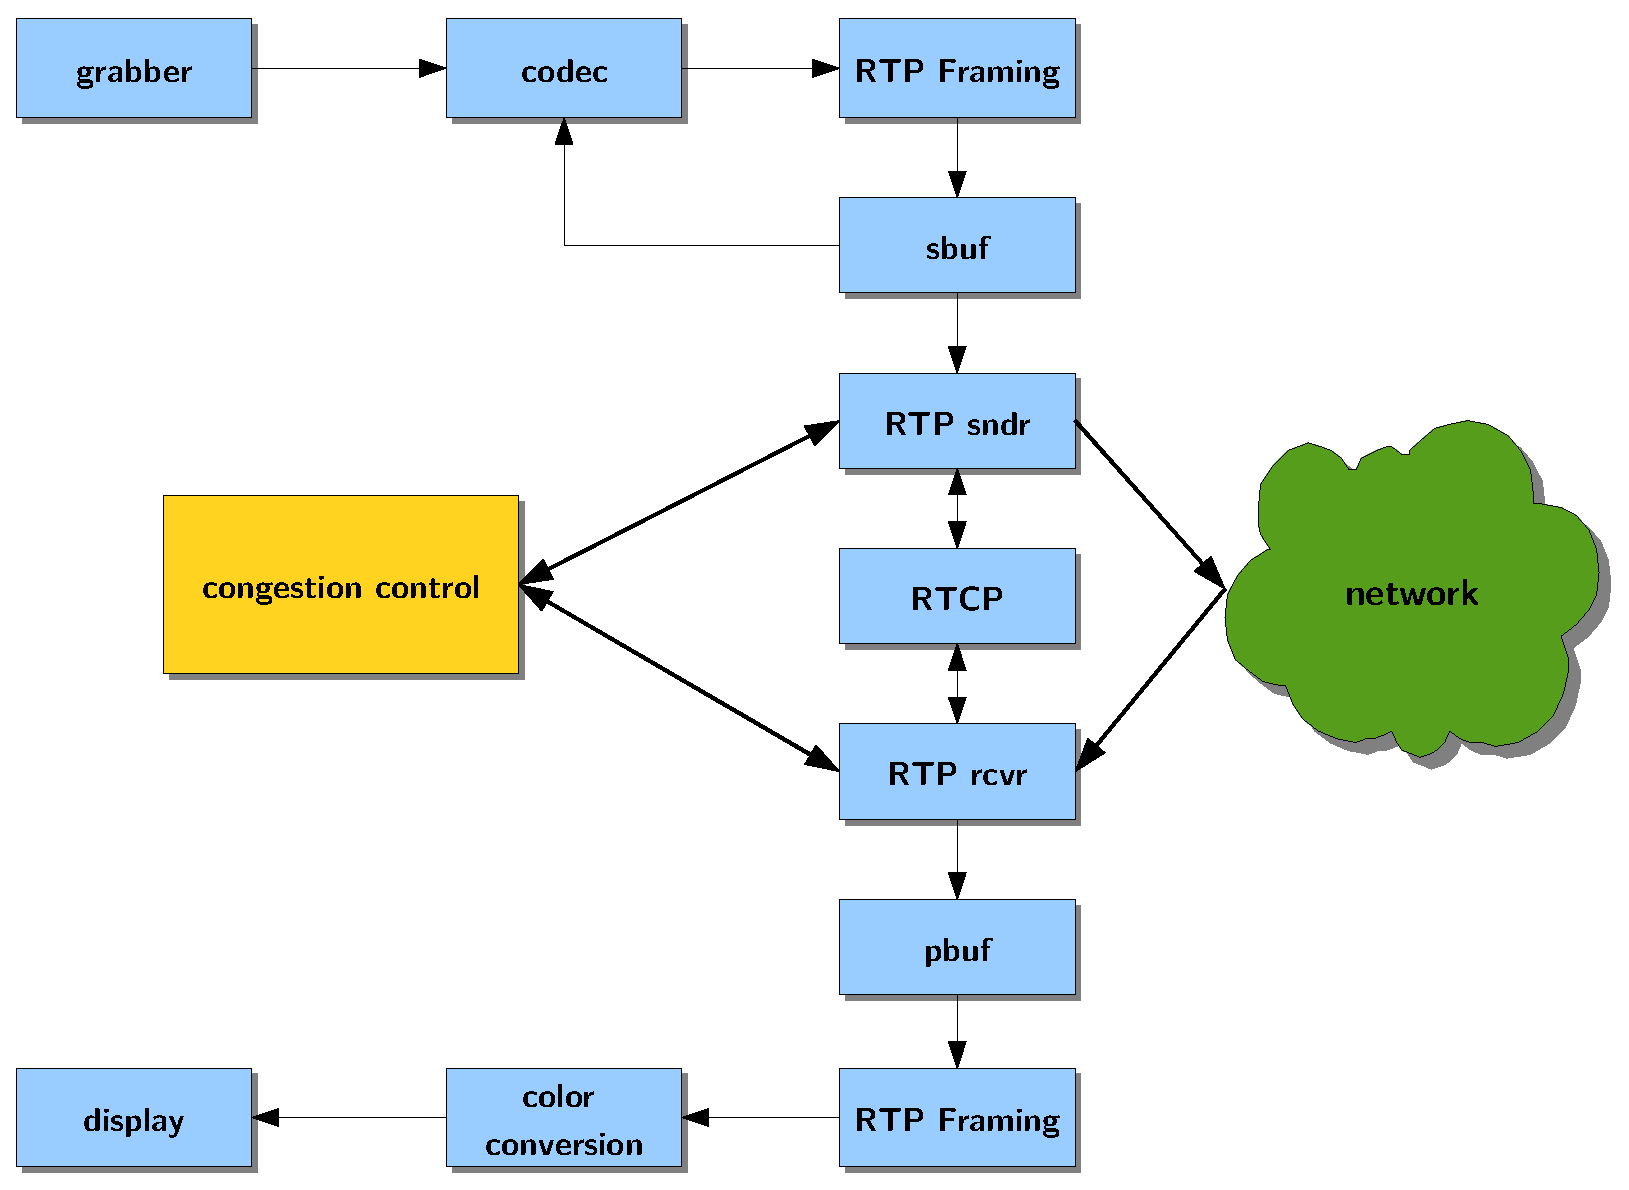
\includegraphics[scale=.5]{./img/ultra-high-arch}
\caption{\label{fig:ultra-high-arch}UltraGrid High-level Architecture}
\end{center}
\end{figure}

\subsection{\label{ssec:ultra-init-all}Initialize All Subsystems}

UltraGrid has 6 subsystems when it gets initialized upon start: 

\begin{itemize}
	\item video codecs (\texttt{init\_video\_codecs()})
	\item video display (\texttt{init\_video\_display()})
	\item video capture (\texttt{init\_video\_capture()})
	\item network (\texttt{init\_network()})
	\item receive (\texttt{init\_receive()})
	\item transmit (\texttt{init\_transmit()})
\end{itemize}

In this report, we would like to focus on \emph{network}, \emph{transmit},
and \emph{video codecs} parts.

\subsubsection{\label{sssec:ultra-init-net}Initialize Network}

Figure~\ref{fig:ultra-init-net} shows the function call flows on its start.

\begin{figure}[!h]
\begin{center}
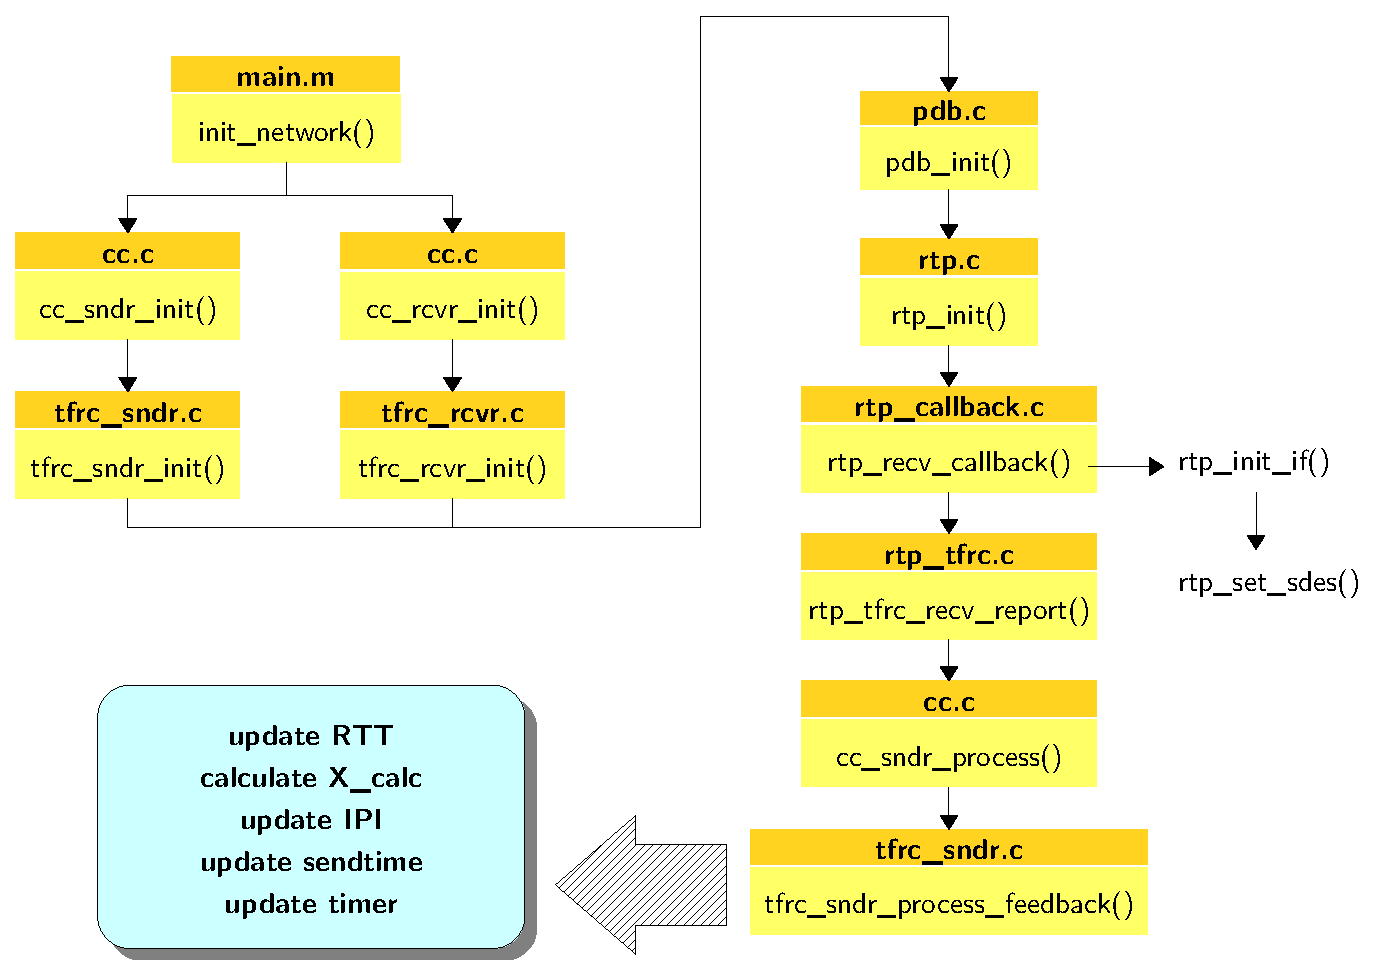
\includegraphics[scale=.6]{./img/ultra-init-net}
\caption{\label{fig:ultra-init-net}Initialize Network}
\end{center}
\end{figure}

\subsubsection{\label{sssec:ultra-init-trans}Initialize Transmit}

Figure~\ref{fig:ultra-init-trans} shows the function call flows.

\begin{figure}[!h]
\begin{center}
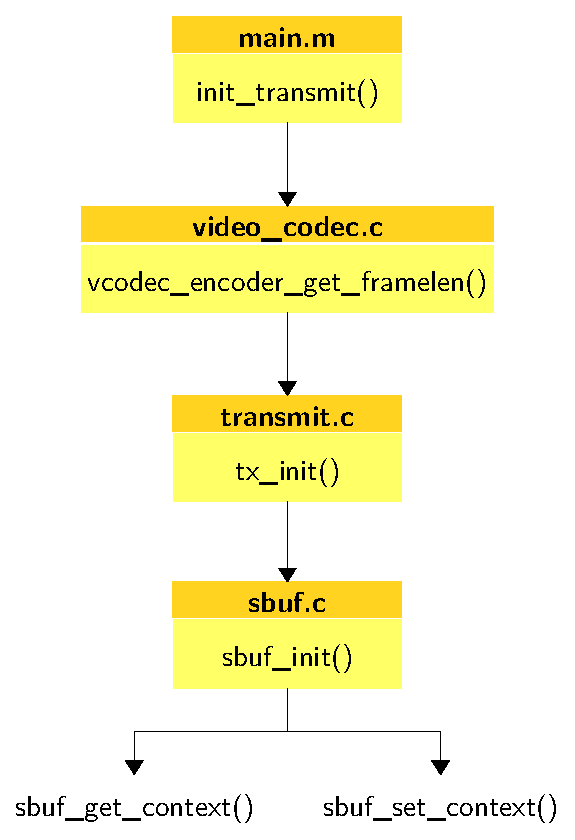
\includegraphics[scale=.6]{./img/ultra-init-trans}
\caption{\label{fig:ultra-init-trans}Initialize Transmit}
\end{center}
\end{figure}


\subsection{\label{ssec:ultra-grab-send}Grab and Send Thread in UltraGrid}

This section shows the grab and send thread in UltraGrid. Note that UltraGrid is
multi-threaded application.

\subsubsection{\label{sssec:ultra-grab}Grab Thread}

Figure~\ref{fig:ultra-grab} shows the function call flows for the grab thread in
UltraGrid.

\begin{figure}[!h]
\begin{center}
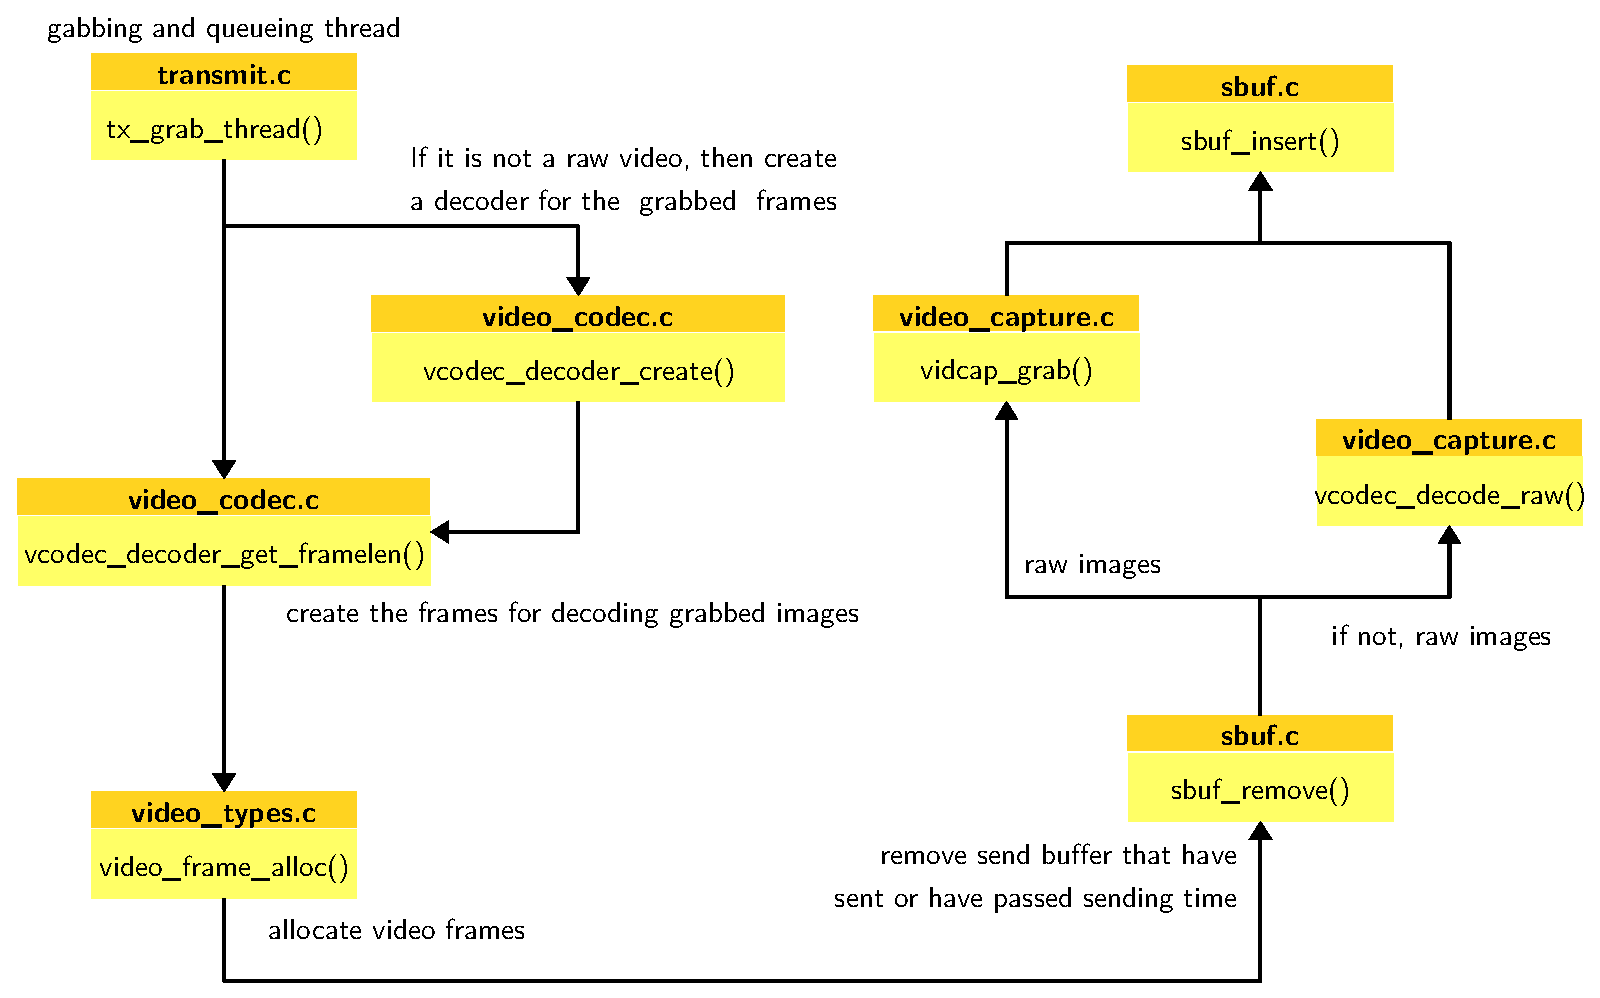
\includegraphics[scale=.5]{./img/ultra-grab}
\caption{\label{fig:ultra-grab}Grab Thread}
\end{center}
\end{figure}

\subsubsection{\label{sssec:ultra-grab}Send Thread} 

Figure~\ref{fig:ultra-send} shows the function call flows for the send thread in
UltraGrid.

\begin{figure}[!h]
\begin{center}
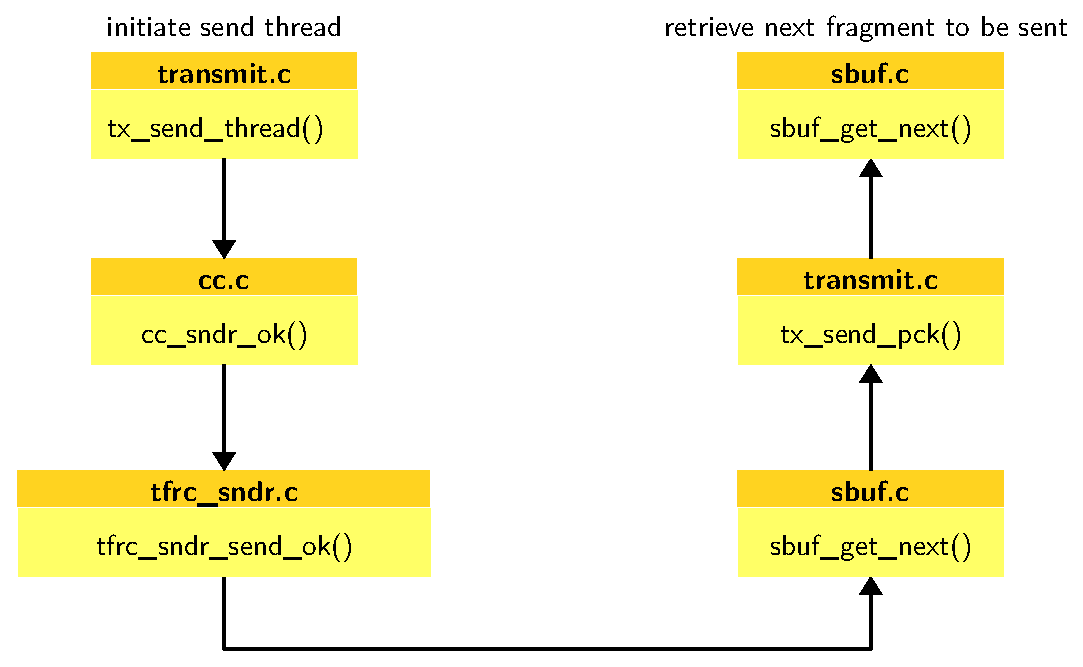
\includegraphics[scale=.5]{./img/ultra-send}
\caption{\label{fig:ultra-send}Send Thread}
\end{center}
\end{figure}

\newpage

